\begin{figure}[htp]
    \centering
    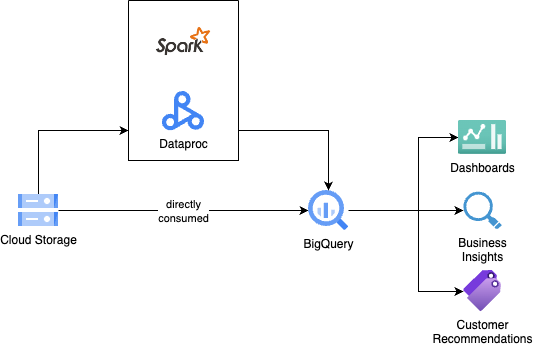
\includegraphics[width=0.5\linewidth]{images/solution_architecture.png}
    \caption{Overview of Solution Architecture}
\end{figure}

As a high-level objective, our team wish to build a dataflow, moving raw data provided by the
retailers into the data warehouse, for which we choose Google BigQuery. After that, within the
warehouse, we perform some transformation to extract value from the retailer inputs. The first one
would be a set of recommendation tag, so called \textbf{Personal Product Ranking} or PPR. Then, we
will visualizing the sale data over the period of the provided time.

To be specific, we will assume that raw data files are uploaded by the retailers to an Object
Storage. Using Google Cloud ecosystem, Cloud Storage is used as the endpoint. About our team
architecture of the solution, we wish to compare between the commonly used Apache Spark for ETL data
from raw files into BigQuery, versus using native BigQuery commands to ingest data. As a result, the
ingestion step from Cloud Storage into BigQuery will be run in two ways. Finally, recommendations
for customers will be stored in a table.

For visualization, to reduce complexity and to promote the full use of BigQuery ecosystem, 